\graphicspath{{/home/arbon/Pictures/Screenshots/}} % path to graphics
\section*{\LARGE{Цель практической работы}}
\addcontentsline{toc}{section}{Цель практической работы}
Получить навыки по работе с командной строкой и git’ом.

\newpage

\section*{\LARGE{Выполнение практической работы}}
\addcontentsline{toc}{section}{Выполнение практической работы}
\section{Установка и настрока клиент git}
\subsection{Установка git}
Установка в Linux и Unix
\begin{itemize}
	\item Используйте обычный менеджер пакетов вашего дистрибутива.
		Откройте терминал и введите подходящие команды.
	\item Если у вас 21 или более ранняя версия Fedora,
		используйте yum install git.
	\item Для 22 и последующих версий Fedora вводите dnf install git.
	\item Для дистрибутивов, основанных на Debian, например, Ubuntu,
		используйте apt-get: sudo apt-get install git.
\end{itemize}
\begin{figure}[h!tp]
	\centering
	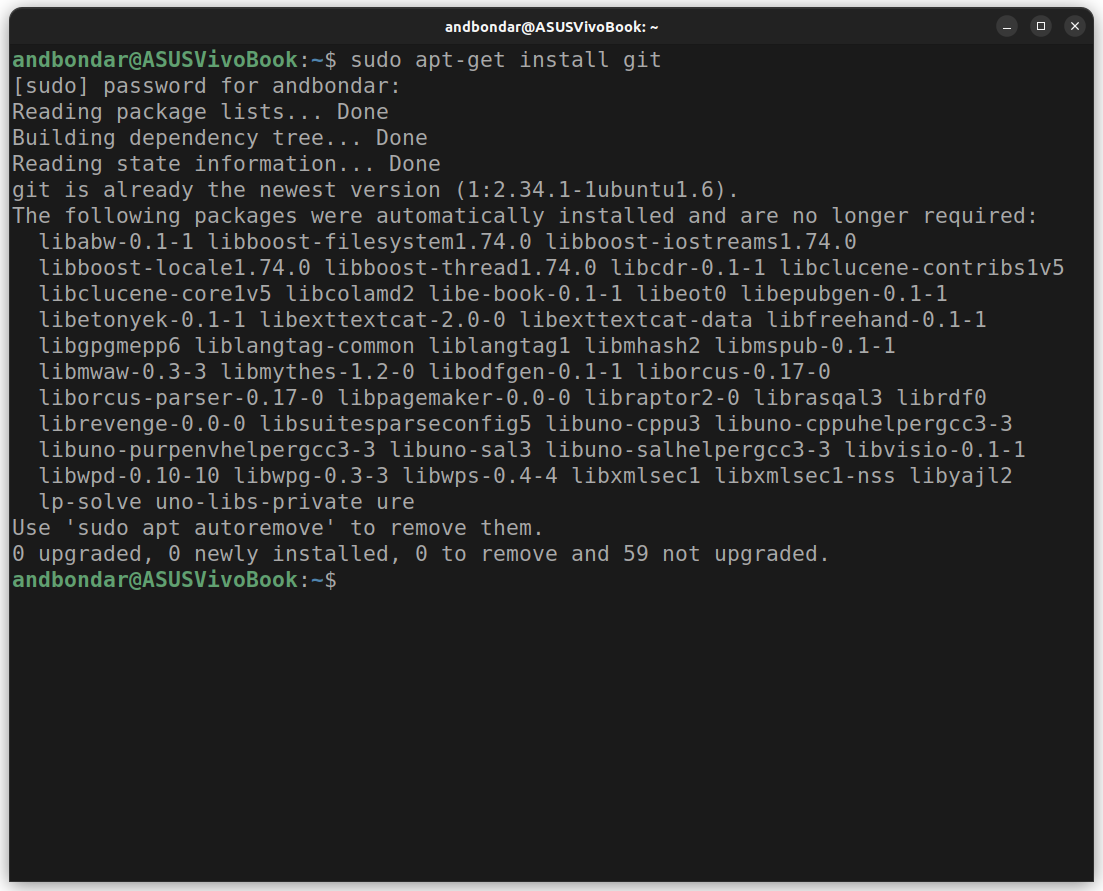
\includegraphics[width=0.7\textwidth]{Screenshot from 2023-02-14 10-47-05.png}
	\caption{Установка git}
	\label{fig:git:install}
\end{figure}

\subsection{Настройка git}
\begin{enumerate}
	\item Открываем терминал.
	\item Необходимо выполнить следующие команды:
	\begin{verbatim}
		git config --global user.name "Your Name"
		git config --global user.email "your_email@whatever.com"
	\end{verbatim}
	\item Необходимо выполнить следующие команды:
	\begin{verbatim}
		git config --global core.autocrlf input
		git config --global core.safecrlf warn
	\end{verbatim}
	\item Необходимо выполнить следующую команды:
	\begin{verbatim}
		git config --global core.quotepath off
	\end{verbatim}
	\item Необходимо выполнить следующую команды:
	\begin{verbatim}
		git config --global core.quotepath off
	\end{verbatim}
\end{enumerate}
Для проверки верности всех введенных команд, введите:
\begin{verbatim}
	git config --list
\end{verbatim}
\begin{figure}[h!tp]
	\centering
	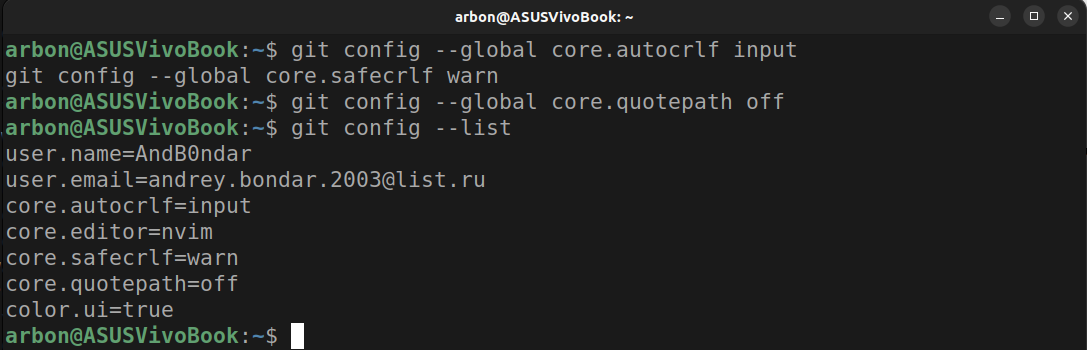
\includegraphics[width=0.8\textwidth]{Screenshot from 2023-02-14 11-05-52.png}
	\caption{Настройка git}
	\label{fig:git:config}
\end{figure}

\section{Создарние локальный репозиторий и добавление в него несколько файлов}
Выполняем команду \texttt{git init}.
После выполнения данной команды, должно высветиться данное сообщение, показанное на рис. \ref{fig:git:init}.
\begin{figure}[h!tp]
	\centering
	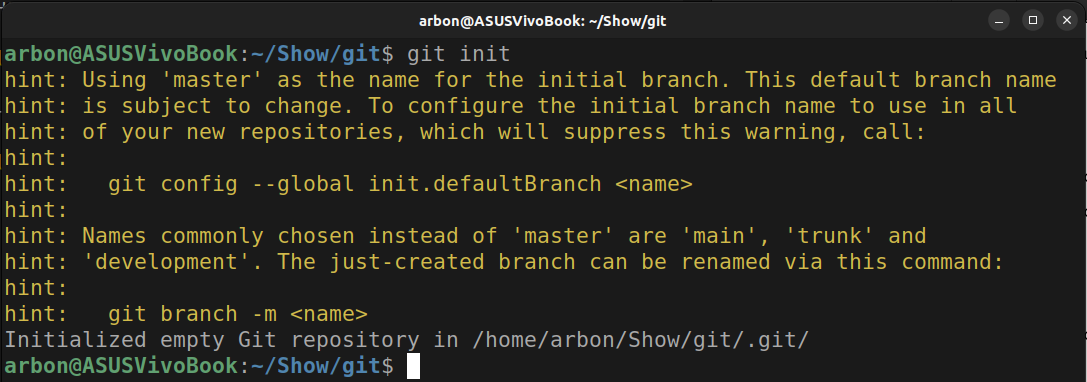
\includegraphics[width=0.8\textwidth]{Screenshot from 2023-02-14 11-21-16.png}
	\caption{Создание репозитория git}
	\label{fig:git:init}
\end{figure}

\section{Добавление файлов в репозиторий}
Далее, командой \texttt{touch file} создадим несколько текстовый файлов.
Чтобы добавить файл в репозиторий необходимо выполнить следующее:
\begin{enumerate}
	\item Вводим команды:
	\begin{verbatim}
		git add <Название вашего файла>
		git commit -m "Ваш текст для коммита"
	\end{verbatim}
\item Чтобы проверить состояние репозитория,
	выполним команду: \texttt{git~status}.
	Команда проверки состояния сообщит, что коммитить нечего.
	Это означает, что в репозитории хранится текущее состояние
	рабочего каталога, и нет никаких изменений, ожидающих записи.
\end{enumerate}
Результат этих действий показан на рисунке \ref{fig:git:first_commit}.
\begin{figure}[h!tp]
	\centering
	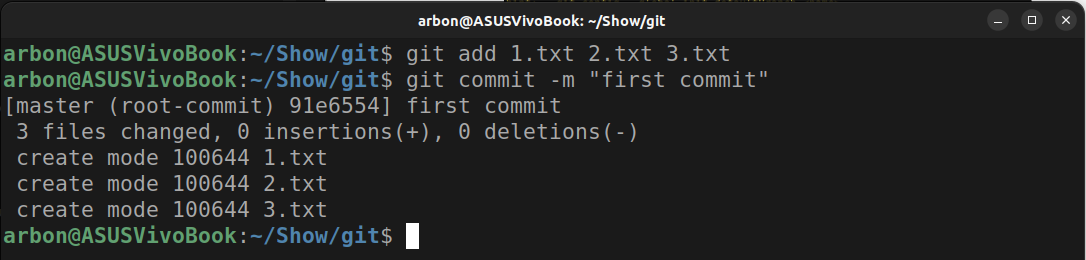
\includegraphics[width=0.8\textwidth]{Screenshot from 2023-02-14 11-32-30.png}
	\caption{Добавление файлов в репозиторий и первый коммит}
	\label{fig:git:first_commit}
\end{figure}

